% !Mode:: "TeX:UTF-8"
\section{LDA}
\maketitle
Gamma函数的定义为:
\begin{displaymath}
\begin{split}
\Gamma(x)=\int_{0}^{\infty}{u^{x-1}e^{-u}du}
\end{split}
\end{displaymath}
Gama函数的性质:
$\Gamma(1)=1; \Gamma(x+1)=x\Gamma(x); \Gamma(x+1) = x!;$

参数为$\vec{A} = (a_1,a_2...a_K)$的Dirichlet分布的定义如下:
\begin{displaymath}
\begin{split}
Dir(\mu|\vec{A})=\frac{\Gamma{(\sum_{k=1}^{K}{a_k}})}{\prod_{k=1}^{K}{\Gamma{(a_k)}}}\prod_{k=1}^{K}{\mu_{k}^{a_k-1}}
\end{split}
\end{displaymath}
给定数据集$D$,$K$个不同类型出现的次数向量$\vec{M}$,当Dirichlet分布作
为先验分布式时:
\begin{displaymath}
\begin{split}
p(\mu|\vec{A},\vec{M})= Dir(\mu|\vec{A}+\vec{M}) = \frac{\Gamma{(\sum_{k=1}^{K}{(a_k+m_k)}})}{\prod_{k=1}^{K}{\Gamma{(a_k+m_k)}}}\prod_{k=1}^{K}{\mu_{k}^{a_k+m_k-1}}
\end{split}
\end{displaymath}
即:给定一个Dirichlet分布的先验和一个多项式分布的条件概率,可以得到一
个Dirichlet分布的一个后验。

\begin{figure}[htbp]
\centering
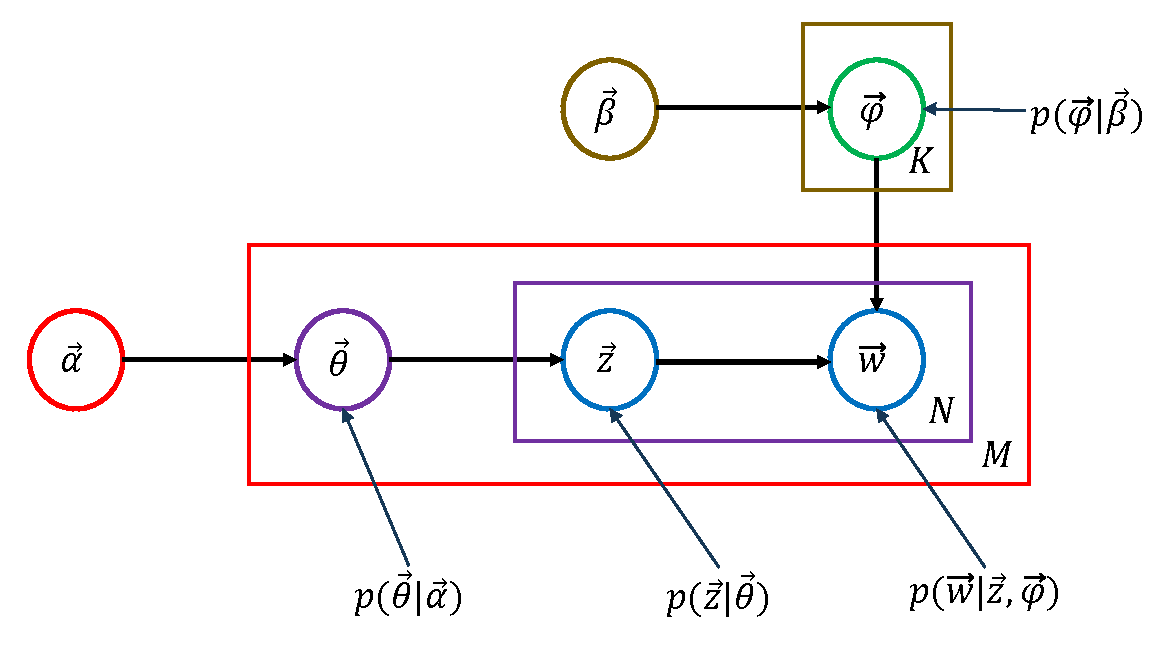
\includegraphics[width = 0.6\textwidth]{LDAFigure}
\end{figure}

整个训练语料库为$\vec{w}$,文档数为$M$,文档$m$中词的个数为$N_m$,则第$m$个文档第$n$词为$w_{m,n}$。
$\vec{w}$的似然函数为:
\begin{displaymath}
\begin{split}
p(\vec{w}|\vec{\alpha}, \vec{\beta}) =
\sum_{\vec{z}}{p(\vec{w}, \vec{z}|\vec{\alpha}, \vec{\beta})}
=\sum_{\vec{z}}{p(\vec{w}|\vec{z},\vec{\beta}) p(\vec{z}|\vec{\alpha})}
\end{split}
\end{displaymath} 

主题数为$K$,词表大小$V$,则主题产生词的概率表$\vec{\phi}$为一个$K
\times V$的一个矩阵,且每个主题($k$)的概率表$\vec{\phi}_k$服从参数为$\vec{\beta}$的Dirichlet
分布:
\begin{displaymath}
\begin{split}
p(\vec{\phi}|\vec{\beta}) &= \prod_{k=1}^{K}{p(\vec{\varphi}_k|\vec{\beta})} 
=\prod_{k=1}^{K}{\frac{\Gamma(\sum_{t=1}^{V}{\beta_t})}{\prod_{t=1}^{V}{\Gamma(\beta_t)}}\prod_{t=1}^{V}{\varphi_{k,t}^{\beta_t-1}}} \\
\end{split}
\end{displaymath} 


给定主题产生词的概率表$\vec{\phi}$以及$M$个文档中所有词的主题编号向量
矩阵$\vec{z}$ (文档数为$M$,文档$m$中词的个数为$N_m$,则第$m$个文档第
$n$词的主题编号为$z_{m,n}$)。矩阵$\vec{z}$跟文档$\vec{w}$是等大小一一
对应的一个矩阵。 $p(\vec{w}|\vec{z},\vec{\phi})$的定义为:
\begin{displaymath}
\begin{split}
p(\vec{w}|\vec{z},\vec{\phi}) 
=\prod_{d=1}^{M}{p(\vec{w}_d|\vec{z}_d, \vec{\phi})} 
=\prod_{d=1}^{M}{\prod_{n=1}^{N_d}{\varphi_{z_{d,n},w_{d,n}}}} 
=\prod_{k=1}^{K}{\prod_{t=1}^{V}{\varphi_{k,t}^{n(k,t)}}}
\end{split}
\end{displaymath}
其中,$\varphi_{z_{d,n},w_{d,n}}$表示第$d$个文档的第$n$个位置的主题
$z_{d,n}$产生词$w_{d,n}$的概率。$n_{k,t}$指的是在所有文档中主题$k$产生
词$t$的次数。

给定$p(\vec{\phi}|\vec{\beta})$和$p(\vec{w}|\vec{z},\vec{\phi})$,则$p(\vec{w}|\vec{z},\vec{\beta})$的定义为:
\begin{displaymath}
\begin{split}
p(\vec{w}|\vec{z},\vec{\beta}) &=
\int{p(\vec{w}|\vec{z},\vec{\phi})p(\vec{\phi}|\vec{\beta})d\vec{\phi}} \\
&= \int{
\prod_{k=1}^{K}{\frac{\Gamma(\sum_{t=1}^{V}{\beta_t})}{\prod_{t=1}^{V}{\Gamma(\beta_t)}}\prod_{t=1}^{V}{\varphi_{k,t}^{\beta_t-1}}}
\cdot
\prod_{k=1}^{K}{\prod_{t=1}^{V}{\varphi_{k,t}^{n(k,t)}}}
d\varphi_{k,t}} \\
&= \int{
\prod_{k=1}^{K}{
    \frac{\Gamma(\sum_{t=1}^{V}{\beta_t})}{\prod_{t=1}^{V}{\Gamma(\beta_t)}}
    \prod_{t=1}^{V}{\varphi_{k,t}^{n(k,t)+\beta_t-1}}
}
d\varphi_{k,t}} \\
&= \int{
\prod_{k=1}^{K}{
    \frac{\triangle(\vec{n}_k+\vec{\beta})}{\triangle(\vec{\beta})}
    \frac{1}{\triangle(\vec{n}_k+\vec{\beta})}
    \prod_{t=1}^{V}{\varphi_{k,t}^{n(k,t)+\beta_t-1}}
}
d\varphi_{k,t}} \Longleftarrow \frac{1}{\triangle(\vec{\beta})}=\frac{\Gamma{(\sum_{t=1}^{V}{\beta_k}})}{\prod_{t=1}^{V}{\Gamma{(\beta_t)}}} \\
&= \prod_{k=1}^{K}{
   \frac{\triangle(\vec{n}_k+\vec{\beta})}{\triangle(\vec{\beta})}
   \underbrace{
   \int{
       \frac{1}{\triangle(\vec{n}_k+\vec{\beta})}
      \prod_{t=1}^{V}{\varphi_{k,t}^{n(k,t)+\beta_t-1}}
    d\varphi_{k,t}}
   }_{\int{Dir(\vec{\varphi}|\vec{n}_k + \vec{\beta})d\vec{\varphi}}=1}
}\\
&= \prod_{k=1}^{K}{ \frac{\triangle(\vec{n}_k+\vec{\beta})}{\triangle(\vec{\beta})}}\\
\end{split}
\end{displaymath} 


文档数为$M$,主题数为$K$,则文档产生主题的概率表$\vec{\theta}$为一个$M
\times K$的矩阵,且第$d$个文档的概率表$\vec{\theta}_d$服从参数为$\vec{\alpha}$的Dirichlet
分布:
\begin{displaymath}
\begin{split}
p(\vec{\theta}|\vec{\alpha}) 
= \prod_{d=1}^{M}{p(\vec{\theta}_d|\vec{\alpha})} 
=\prod_{d=1}^{M}{\frac{\Gamma(\sum_{k=1}^{K}{\alpha_k})}{\prod_{k=1}^{K}{\Gamma(\alpha_k)}}\prod_{k=1}^{K}{\theta_{d,k}^{\alpha_k-1}}} \\
\end{split}
\end{displaymath} 


给定文档产生主题的概率表$\vec{\theta}$, $p(\vec{z}|\vec{\theta})$的定义为:
\begin{displaymath}
\begin{split}
p(\vec{z}|\vec{\theta})
= \prod_{d=1}^{M}{p(\vec{z}_d|\vec{\theta}_d)}
= \prod_{d=1}^{M}{\prod_{n=1}^{N_d}{\theta_{d,z_{d,n}}}}
=\prod_{d=1}^{M}{\prod_{k=1}^{K}{\theta_{d,k}^{n(d,k)}}}
\end{split}
\end{displaymath}
其中,$z_{d,n}$是第$d$个文档第$n$个单词的主题。$\vec{\theta}$中存放
了$d$个文档产生主题$z_{d,n}$的概率$\theta_{d,z_{d,n}}$。$n(d,k)$表示
第$d$个文档中词的主题是$k$的个数。

给定$\vec{\theta}$和$p(\vec{z}|\vec{\theta})$,则$p(\vec{z}|\vec{\alpha})$的定义为:
\begin{displaymath}
\begin{split}
p(\vec{z}|\vec{\alpha}) 
&= \int{p(\vec{z}|\vec{\theta})p(\vec{\theta}|\vec{\alpha})d\vec{\theta}}\\
&= \int{
     \prod_{d=1}^{M}{\frac{\Gamma(\sum_{k=1}^{K}{\alpha_k})}{\prod_{k=1}^{K}{\Gamma(\alpha_k)}}\prod_{k=1}^{K}{\theta_{d,k}^{\alpha_k-1}}}
     \cdot
     \prod_{d=1}^{M}{\prod_{k=1}^{K}{\theta_{d,k}^{n(d,k)}}}
d\vec{\theta}_{d,k}}\\
&= \int{
     \prod_{d=1}^{M}{\frac{\Gamma(\sum_{k=1}^{K}{\alpha_k})}{\prod_{k=1}^{K}{\Gamma(\alpha_k)}}
       \prod_{k=1}^{K}{\theta_{d,k}^{n(d,k)+\alpha_k -1}}
     }
d\vec{\theta}_{d,k}}\\
&= \int{
     \prod_{d=1}^{M}{
       \frac{\triangle(\vec{n}_d+\vec{\alpha})}{\triangle(\vec{\alpha})}
       \frac{1}{\triangle(\vec{n}_d+\vec{\alpha})}
       \prod_{k=1}^{K}{\theta_{d,k}^{n(d,k)+\alpha_k -1}}
     }
d\vec{\theta}_{d,k}}\\
&= \prod_{d=1}^{M}{\frac{\triangle(\vec{n}_d+\vec{\alpha})}{\triangle(\vec{\alpha})}
\underbrace{
    \int{
       \frac{1}{\triangle(\vec{n}_d+\vec{\alpha})}
       \prod_{k=1}^{K}{\theta_{d,k}^{n(d,k)+\alpha_k -1}}
     d\vec{\theta}_{d,k}}
}_{\int{Dir(\vec{\theta}|\vec{n}_d + \vec{\alpha})d\vec{\theta}}=1}
}\\
&= \prod_{d=1}^{M}{\frac{\triangle(\vec{n}_d+\vec{\alpha})}{\triangle(\vec{\alpha})}}\\
\end{split}
\end{displaymath} 

$\vec{w}$的似然函数为:
\begin{displaymath}
\begin{split}
p(\vec{w}|\vec{\alpha}, \vec{\beta}) 
&= \sum_{\vec{z}}{
  p(\vec{w}|\vec{z},\vec{\beta})p(\vec{z}|\vec{\alpha})}\\
&= \sum_{\vec{z}}{(
    \prod_{k=1}^{K}{
        \frac{\triangle(\vec{n}_k+\vec{\beta})}{\triangle(\vec{\beta})}
    }
    \cdot
    \prod_{d=1}^{M}{
        \frac{\triangle(\vec{n}_d+\vec{\alpha})}{\triangle(\vec{\alpha})}
    }
)}\\
&= \sum_{\vec{z}}{(
\prod_{k=1}^{K}{
     {
     \frac{\prod_{t=1}^{V}{\Gamma{((\vec{n}_k+\vec{\beta})_t)}}}{\Gamma{(\sum_{t=1}^{V}{(\vec{n}_k+\vec{\beta})_t})}}
     }
      \cdot
     {
      \frac{\Gamma{(\sum_{t=1}^{V}{\vec{\beta}_t})}}{\prod_{t=1}^{V}{\Gamma{(\vec{\beta}_t)}}}
     }
}
\cdot
\prod_{d=1}^{M}{
     {
      \frac{\prod_{k=1}^{K}{\Gamma((\vec{n}_d+\vec{\alpha})_k)}}{\Gamma(\sum_{k=1}^{K}{(\vec{n}_d+\vec{\alpha})_k}}
     }
\cdot
     { 
      \frac{\Gamma(\sum_{k=1}^{K}{\alpha_k})}{\prod_{k=1}^{K}{\Gamma(\alpha_k)}}
     }
}
)}
\end{split}
\end{displaymath} 
其中,待优化参数为$\vec{n}_k$和$\vec{n}_d$。$\vec{n}_k$是主题$k$产生单
词的计数表,总共有$K$个不同的$\vec{n}_k$,每个$\vec{n}_k$的维度为词表
大小。$\vec{n}_d$是文档$d$产生主题的计数表,总共有$M$个不同的
$\vec{n}_d$,每个$\vec{n}_d$的维度为主题数。


为了能够进行采样,我们需要计算产生第$i=(m,n)$个词(即:第$m$个文档的第
$n$个词)的主题为$k$的条件概
率:$p(z_i=k|\vec{z}_{\neg i}, \vec{w},\vec{\alpha}, \vec{\beta})$.我们定
义如下符号:
$\vec{n}_{k, \neg i}$ 表示将主题为$k$的主题到词的计数$\vec{n}_k$中把第$i$个
词的计数删掉。故而 $(\vec{n}_{k}+\vec{\beta})_i = (\vec{n}_{k, \neg i}+\vec{\beta})_i + 1$,从而有:
\begin{displaymath}
\begin{split}
\frac{\Gamma(\sum_{t=1}^{V}{(\vec{n}_{k, \neg i}+\vec{\beta})_t})  }{ 
       \Gamma(\sum_{t=1}^{V}{(\vec{n}_{k}+\vec{\beta})_t})} 
&= \frac{
     \Gamma(\sum_{t=1; t \neq i}^{V}{(\vec{n}_{k}+\vec{\beta})_t}  
       + (\vec{n}_{k, \neg i}+\vec{\beta})_i)
}{ \Gamma(\sum_{t=1; t \neq i}^{V}{(\vec{n}_{k}+\vec{\beta})_t}
    + (\vec{n}_{k}+\vec{\beta})_i
)} \\
&=  \frac{
     \Gamma(\sum_{t=1; t \neq i}^{V}{(\vec{n}_{k}+\vec{\beta})_t}  
       + (\vec{n}_{k, \neg i}+\vec{\beta})_i)
}{ \Gamma(\sum_{t=1; t \neq i}^{V}{(\vec{n}_{k}+\vec{\beta})_t}
    + (\vec{n}_{k, \neg i}+\vec{\beta})_i +1
)} \\
&=  \frac{1}{\sum_{t=1; t \neq i}^{V}{(\vec{n}_{k}+\vec{\beta})_t}
    + (\vec{n}_{k, \neg i}+\vec{\beta}_i)
} =  \frac{1}{\sum_{t=1}^{V}{(\vec{n}_{k, \neg i}+\vec{\beta})_t}
} \\
\end{split}
\end{displaymath}
同样的$\vec{n}_{m, \neg i}$表示在第$m$个文档中产生词的主题的计数$\vec{n}_m$中把第$i$个
词对应的主题计数删掉。故而 $(\vec{n}_{m}+\vec{\alpha})_k =
(\vec{n}_{m, \neg i}+\vec{\alpha})_k + 1$,从而有:
\begin{displaymath}
\begin{split}
\frac{ \Gamma(\sum_{k'=1}^{K}{(\vec{n}_{m, \neg i}+\vec{\alpha})_{k'}})
}{     \Gamma(\sum_{k'=1}^{K}{(\vec{n}_{m}+\vec{\alpha})_{k'}}) 
}
&=  \frac{1}{\sum_{k'=1}^{K}{(\vec{n}_{m, \neg i}+\vec{\alpha})_{k'}}
} \\
\end{split}
\end{displaymath}

$p(\vec{w}_{\neg i}| \vec{z_{\neg i}}, \vec{\alpha},\vec{\beta})$ 和
$p(\vec{z}_{\neg i}|\vec{\alpha}, \vec{\beta})$ 表示将第$i=(m,n)$个词
删掉,从而产生一个新的语料。新的语料同原始语料的区别仅仅在于第$m$个文
档中不包含第$n$个词,故而其产生过程中也不需要生成对应的$z_i$。我们记第
$i$个term 的 ID为$t$,第$i$个词的主题为$k$。
\begin{displaymath}
\begin{split}
p(\vec{w}_{\neg i}| \vec{z_{\neg i}}, \vec{\beta}) &= 
\prod_{k'=1;k' \neq k}^{K}{
       \frac{\triangle(\vec{n}_{k'}+\vec{\beta})}
            {\triangle(\vec{\beta})}})
\cdot
 \frac{\triangle(\vec{n}_{k, \neg i}+\vec{\beta})}
      {\triangle(\vec{\beta})}\\
p(\vec{z}_{\neg i}|\vec{\alpha}) &=
\prod_{d=1; d \neq m}^{M}{\frac{\triangle(\vec{n}_d+\vec{\alpha})}
                  {\triangle(\vec{\alpha})}}
       \cdot
\frac{\triangle(\vec{n}_{m; \neg i}+\vec{\alpha})}
     {\triangle(\vec{\alpha})}
\end{split}
\end{displaymath}

\begin{displaymath}
\begin{split}
p(z_i=k|\vec{z}_{\neg i}, \vec{w}, \vec{\alpha}, \vec{\beta}) &=
\frac{ p(\vec{w}, \vec{z}|\vec{\alpha}, \vec{\beta}) }
     { p(\vec{w}, \vec{z_{\neg i}}|\vec{\alpha}, \vec{\beta})}\\
&=\frac{ p(\vec{w}| \vec{z}, \vec{\alpha}, \vec{\beta})
         p(\vec{z}| \vec{\alpha}, \vec{\beta})  }
     { p(\vec{w}_{\neg i}| \vec{z_{\neg i}},\vec{\alpha},\vec{\beta})
        p(\vec{z_{\neg i}}|\vec{\alpha},\vec{\beta})
      p(w_i|\vec{z}_{\neg i}, \vec{\alpha}, \vec{\beta})} \\
&= \frac{ p(\vec{w}| \vec{z}, \vec{\beta}) }
     { p(\vec{w}_{\neg i}| \vec{z_{\neg i}}, \vec{\beta})p(w_i|\vec{\alpha}, \vec{\beta})}
\cdot
\frac{p(\vec{z}|\vec{\alpha})}{p(\vec{z}_{\neg
    i}|\vec{\alpha})}
\\
&\propto  \frac{ p(\vec{w}| \vec{z}, \vec{\beta}) }
     { p(\vec{w}_{\neg i}| \vec{z_{\neg i}}, \vec{\beta})}
\cdot
\frac{p(\vec{z}|\vec{\alpha})}{p(\vec{z}_{\neg i}|\vec{\alpha})}
\Longleftarrow p(w_i|\vec{\alpha}, \vec{\beta})=C
\\
&=  \frac{
      \prod_{k'=1}^{K}{\frac{\triangle(\vec{n}_{k'}+\vec{\beta})}
                   {\triangle(\vec{\beta})}} 
    }
     {(\prod_{k'=1;k' \neq k}^{K}{
       \frac{\triangle(\vec{n}_{k'}+\vec{\beta})}
            {\triangle(\vec{\beta})}})
      \cdot
       \frac{\triangle(\vec{n}_{k, \neg i}+\vec{\beta})}
            {\triangle(\vec{\beta})}
      }
\cdot
\frac{
     \prod_{d=1}^{M}{\frac{\triangle(\vec{n}_d+\vec{\alpha})}
                  {\triangle(\vec{\alpha})}}
     }{
       \prod_{d=1; d \neq m}^{M}{\frac{\triangle(\vec{n}_d+\vec{\alpha})}
                  {\triangle(\vec{\alpha})}}
       \cdot
       \frac{\triangle(\vec{n}_{m; \neg i}+\vec{\alpha})}
            {\triangle(\vec{\alpha})}
}\\
&= \frac{ \triangle(\vec{n}_{k}+\vec{\beta}) }
        { \triangle(\vec{n}_{k, \neg i}+\vec{\beta})
        }
\cdot
\frac{\triangle(\vec{n}_{m}+\vec{\alpha})
     }{\triangle(\vec{n}_{m; \neg i}+\vec{\alpha})
}\\
&= \frac{\Gamma(\sum_{t'=1}^{V}{(\vec{n}_{k, \neg i}+\vec{\beta})_{t'}})
        \cdot
        \prod_{t'=1}^{V}{ \Gamma((\vec{n}_{k}+\vec{\beta})_{t'}) }
        }{
       \prod_{t'=1}^{V}{ \Gamma((\vec{n}_{k, \neg i}+\vec{\beta})_{t'}) }
       \cdot
       \Gamma(\sum_{t'=1}^{V}{(\vec{n}_{k}+\vec{\beta})_{t'}})
}\\
&\cdot
\frac{ \Gamma(\sum_{k'=1}^{K}{(\vec{n}_{m, \neg i}+\vec{\alpha})_{k'}})
       \cdot
        \prod_{k'=1}^{K}{ \Gamma(\vec{n}_{m}+\vec{\alpha})_{k'} }
}{     \Gamma(\sum_{k'=1}^{K}{(\vec{n}_{m}+\vec{\alpha})_{k'}})
        \cdot
       \prod_{k'=1}^{K}{ \Gamma(\vec{n}_{m, \neg i}+\vec{\alpha})_{k'} }
}\\
&= \frac{\prod_{t'=1}^{V}{  \Gamma((\vec{n}_{k}+\vec{\beta})_{t'})  }
        }{
       \prod_{t'=1}^{V}{ \Gamma((\vec{n}_{k, \neg i}+\vec{\beta})_{t'}) }
       \cdot
       \sum_{t'=1}^{V}{(\vec{n}_{k, \neg i}+\vec{\beta})_{t'}}
       }\\
&\cdot
\frac{ \prod_{k'=1}^{K}{ \Gamma(\vec{n}_{m}+\vec{\alpha})_{k'}}
}{     \prod_{k'=1}^{K}{ \Gamma(\vec{n}_{m, \neg i}+\vec{\alpha})_{k'}}
        \cdot
        \sum_{k'=1}^{K}{(\vec{n}_{k', \neg i}+\vec{\alpha})_{k'}}
}\\
&= \frac{\Gamma((\vec{n}_{k}+\vec{\beta})_t)
        }{
       \Gamma((\vec{n}_{k, \neg i}+\vec{\beta})_t)
       \cdot
       \sum_{t'=1}^{V}{(\vec{n}_{k, \neg i}+\vec{\beta})_{t'}}
       }\\
&\cdot
\frac{\Gamma((\vec{n}_{m}+\vec{\alpha})_{k})
}{ \Gamma((\vec{n}_{m, \neg i}+\vec{\alpha})_{k})
        \cdot
        \sum_{k'=1}^{K}{(\vec{n}_{k', \neg i}+\vec{\alpha})_{k'}}
}\\
&= \frac{(\vec{n}_{k, \neg i}+\vec{\beta})_t
        }{
       \sum_{t'=1}^{V}{(\vec{n}_{k, \neg i}+\vec{\beta})_{t'}}
       }
\cdot
\frac{((\vec{n}_{m, \neg i}+\vec{\alpha})_{k}
}{\sum_{k'=1}^{K}{(\vec{n}_{k', \neg i}+\vec{\alpha})_{k'}}
}\\
\end{split}
\end{displaymath}

由Dirichlet分布的期望公式得:
\begin{displaymath}
\begin{split}
 \hat{\varphi}_{kt} &= \frac{(\vec{n}_{k, \neg i}+\vec{\beta})_t
        }{
       \sum_{t'=1}^{V}{(\vec{n}_{k, \neg i}+\vec{\beta})_{t'}}
       }
\\
\hat{\theta}_{mk} &= \frac{((\vec{n}_{m, \neg i}+\vec{\alpha})_{k}
}{\sum_{k'=1}^{K}{(\vec{n}_{k', \neg i}+\vec{\alpha})_{k'}}
}
\end{split}
\end{displaymath}

给定$\vec{\alpha}$作为先验,我们使用模型来产生了一批数据,这批数
据除了没有产生第$m$个文档的第$n$个词,其余同原始数据一样,即
$\vec{z}_{\neg i}$以及$\vec{w}_{\neg i}$,那么$\vec{\theta}_m$
的后验概率仍然为一个$Dir$概率分布,故而有$p(\vec{\theta}_m|\vec{z}_{\neg i}, \vec{w}_{\neg i}) = Dir(\vec{\theta}_m|\vec{n}_{m, \neg i} + \vec{\alpha})$。同理
$p(\vec{\varphi}_k|\vec{z}_{\neg i}, \vec{w}_{\neg i}) =
Dir(\vec{\varphi}_k|\vec{n}_{k, \neg i}+\vec{\beta})$。基于这两个公式,
我们可以用另一个方法进行证明:
\begin{displaymath}
\begin{split}\
p(z_i=k|\vec{z}_{\neg i}, \vec{w})  
&= p(z_i=k|\vec{z}_{\neg i},w_i=t, \vec{w}_{\neg i})  \\
&=\frac{p(z_i=k, w_i=t|\vec{z}_{\neg i}, \vec{w}_{\neg i})}{p(w_i = t)}\\
&\propto
p(z_i=k,w_i=t|\vec{z}_{\neg i}, \vec{w}_{\neg i})\\
&=\int{p(z_i=k, w_i=t, \vec{\theta}_m, \vec{\varphi}_k|\vec{z}_{\neg i},
\vec{w}_{\neg i})}d\vec{\theta}_md\vec{\varphi}_k\\
&=\int{p(z_i=k, \vec{\theta}_m|\vec{z}_{\neg i},
\vec{w}_{\neg i})
p(w_i=t, \vec{\varphi}_k|\vec{z}_{\neg i},
\vec{w}_{\neg i})}d\vec{\theta}_md\vec{\varphi}_k\\
&=\int{p(z_i=k|\vec{\theta}_m)
p(\vec{\theta}_m|\vec{z}_{\neg i}, \vec{w}_{\neg i})
p(w_i=t| \vec{\varphi}_k)
p(\vec{\varphi}_k|\vec{z}_{\neg i}, \vec{w}_{\neg i})
}d\vec{\theta}_md\vec{\varphi}_k\\
&=\int{p(z_i=k|\vec{\theta}_m)
p(\vec{\theta}_m|\vec{z}_{\neg i}, \vec{w}_{\neg i})
}d\vec{\theta}_m
\int{p(w_i=t| \vec{\varphi}_k)
p(\vec{\varphi}_k|\vec{z}_{\neg i}, \vec{w}_{\neg i})
}d\vec{\varphi}_k\\
&=\int{p(z_i=k|\vec{\theta}_m)
Dir(\vec{\theta}_m|\vec{n}_{m, \neg i} + \vec{\alpha})
}d\vec{\theta}_m 
 \cdot \int{
p(w_i=t| \vec{\varphi}_k)
Dir(\vec{\varphi}_k|\vec{n}_{k, \neg i}+\vec{\beta})
}d\vec{\varphi}_k\\
&=\int{\theta_{mk}
Dir(\vec{\theta}_m|\vec{n}_{m, \neg i} + \vec{\alpha})
}d\vec{\theta}_m  \cdot \int{
\varphi_{kt}
Dir(\vec{\varphi}_k|\vec{n}_{k, \neg i}+\vec{\beta})
}d\vec{\varphi}_k\\
&= \mathbf{E}(\theta_{mk}) \cdot \mathbf{E}(\varphi_{kt})\\
&= \hat{\theta}_{mk} \cdot \hat{\varphi}_{kt}
\end{split}
\end{displaymath}


\begin{minipage}{0.8\textwidth}\centering
\begin{algorithm}[H]
$\boxdot$ initialization:\\
zero all count variables, $n_m^{(k)}$, $n_m$, $n_k^{(t)}$, $n_k$\\
\For{all documents $m \in [1,M]$}{
  \For{all words $n \in [1, N_m]$ in document $m$}{
      sample topic index $z_{m,n}=k \sim Mult(1/K)$\\
      increment document-topic count:$n_m^{(k)}+1$\\
      increment document-topic sum: $n_m + 1$\\
      increment topic-term count: $n_k^{(t)}+1$\\
      increment topic-term sum: $n_k+1$\\
  }
}
$\boxdot$ Gibbs sampling over burn-in period and sampling period:\\
\While{not finished}
{
  \For{all documents $m \in [1,M]$}{
    \For{all words $n \in [1, N_m]$ in document $m$}{
      $\boxdot$ for the current assignment of $k$ to a term $t$ for word $w_{m,n}$:\\
      decrement counts and sums: $n_m^{(k)}-1$, $n_m-1$, $n_k^{(t)}-1$,
      $n_k-1$;\\
      $\boxdot$ multinomial sampling (decrements from previous step):\\
      sample topic index $\tilde{k} \sim p(z_i|\vec{z}_{\neg i}, \vec{w})$;\\
      $\boxdot$ use the new assignment of $z_{m,n}$ to the term $t$ for word
      $w_{m,n}$:\\
      increment counts and sums: $n_m^{(\tilde{k})}-1$, $n_m-1$, $n_{\tilde{k}}^{(t)}-1$, $n_{\tilde{k}}-1$;
    }
  }
   $\boxdot$ Check convergence and read out parameters:\\
   \If{converged and $L$ sampling iterations since last read out}
   {
      $\boxdot$ the different parameters read outs are averaged:\\
      read out parameters set $\vec{\phi}$\\
      read out parameters set $\vec{\theta}$
  }
}
\end{algorithm}
\end{minipage}
